\documentclass[documentclass]{jsarticle}
\usepackage[top=25truemm,bottom=25truemm,left=20truemm,right=20truemm]{geometry}
\usepackage{listings, jlisting, color}
\usepackage[dvipdfmx]{graphicx}
\usepackage{pdfpages}
\usepackage{amsmath}
\usepackage{amssymb, latexsym}
\usepackage{mathtools}
\usepackage{multirow}
\usepackage{color}
\usepackage{ulem}
\usepackage{here}
\usepackage{wrapfig}
\usepackage{tikz}
\usepackage{tcolorbox}
\tcbuselibrary{breakable, skins, theorems}

% 使用する関数の宣言
% (最低限これさえ宣言していれば十分だと思われるものを書いています)
\usetikzlibrary{intersections, calc, arrows, positioning, arrows.meta}


\newcommand{\Add}[1]{\textcolor{red}{#1}}
\newcommand{\Erase}[1]{\textcolor{red}{\sout{\textcolor{black}{#1}}}}
\newcommand{\ctext}[1]{\raise0.2ex\hbox{\textcircled{\scriptsize{#1}}}}

\lstset{
  basicstyle={\small},
  breaklines=true,
  frame=single,
  tabsize=3,
  numbers=left
}

\begin{document}
\title{ソフトウェア設計演習 設計演習2}
\author{222C1021 今村優希}
\maketitle

%\tableofcontents
\clearpage

\newpage

\section{今回のシステム}

今回は下記仕様の「スクールバスシステム」に対して機能を拡張したシステムを作成した.


\begin{tcolorbox}
  利用者は、スクールバスを利用するためにチケットを購入する。
  チケットには回数券と月利用券がある。
  チケットは電子的なものであり、システムで管理し、スマホで確認可能とする。
  購入は大学生協アプリもしくはクレジットカードを使用する(どちらも外部システムを利用する)。
  スクールバスを利用する際には、乗車時と降車時にスマホをかざし記録を取る。
  スクールバスのダイヤは、大学の事務が登録し、利用者は閲覧できる。
\end{tcolorbox}

新規に追加した機能の概要は,
\begin{tcolorbox}
  利用者は運行中のスクールバスの位置を一覧で確認することができる.
\end{tcolorbox}
というものである.
具体的な動作としては,利用者は現在運行中のバスがどこにいるのかを一覧で確認することができる.
現在地は緯度経度で保存され,利用者はその情報をもとに外部の地図等を用いて視覚的に確認することができる.
今回のシステムは,緯度経度を渡すのみで,地図に表示するということを考えない.
スクールバス側は現在の緯度経度をサーバーに通知し,サーバーは利用者に位置を伝える.

\section{システムの作成手順}

今回のシステムは,前回作成したシステムの概要を元に作成を行った.
ただ,複数回の授業を通して訂正,修正を必要とする箇所があったため,ユースケース図,クラス図から再度作成をし直した.
作成する上では下記の順番でUML図を作成し,その図を作成し終わると同時にレビューを実施し,後の工程に影響が出ないよう工夫した.
\begin{itemize}
  \item ユースケース図/記述
  \item クラス図
  \item シーケンス図
  \item アクティビティ図
  \item ステートマシン図
\end{itemize}

\newpage

\section{ユースケース図}
システムの概要を把握するためにユースケース図を作成した.
\subsection*{作成}
今回のシステムの内容から,必要なアクターは
\begin{itemize}
  \item 利用者
  \item スクールバス
  \item ダイヤ登録者
  \item チケット購入補助
\end{itemize}
であると考えた.
利用者は「乗車・下車する」「チケットを購入する」「ダイヤを閲覧する」「バス位置を確認する」
のユースケースが存在すると考えた.
また,「乗車・下車する」と同時に記録を取ることから「乗降の記録を取る」というユースケースをincludeした.
「チケットを購入する」に対しては,「チケットを管理する」というユースケースにincludeさせた.
さらに,「チケットを管理する」際に乗降の記録が必要であろうと考え,「乗降の記録を取る」をextendさせた.
スクールバスは,利用者がバスの位置を確認するために「バスの位置を保存する」というユースケースを作成した.
チケット購入補助は,チケットの購入を補助する外部システムを指す.そのため,「チケットを購入」に関連している.
ダイヤ登録者は,「ダイヤ作成」のユースケースに関連している.

各ユースケースの動作はユースケース記述を参考にしてほしい.

結果として作成したユースケースは以下の通りである.
o1,o2は追加の機能を実現するために拡張した部分である.
\begin{itemize}
  \item[1] 乗車・下車する
  \item[2] チケットを購入する
  \item[3] ダイヤを閲覧する
  \item[4] ダイヤを登録する
  \item[5] 乗降の記録を取る
  \item[6] チケットを管理する
  \item[o1] バスの位置を確認する
  \item[o2] バスの位置を保存する       
\end{itemize}

\subsection*{レビュー結果メモ}
\begin{itemize}
  \item ユースケースが多く詳細過ぎると思ったので,一部ユースケースを統合した.
  \item アクターとして「外部システム」という名称でアクターを追加していたが,
  何の役割があるのかはっきりしていなかったため,「チケット購入補助」に名称を変更した.
  \item アクターとして「サーバー」を追加していたが,システム内に組み込まれていると把握したので削除した.
\end{itemize}

\subsection*{作成結果}
これらの考えのもと作成したユースケース記述が図である.
付け加えた機能のために考えたユースケースを青で表示した.

%ユースケース図の作成結果
\begin{figure}[H]
  \begin{center}
    \includegraphics*[scale=0.4]{figure/3-1.png}
  \end{center}
  \caption{ユースケース図}
  \label{fig:3-1}
\end{figure}
\newpage

\section{ユースケース記述}
上記で作成したユースケースすべてに対してユースケース記述の作成を行った.
\subsection*{概要と作成結果}
\subsubsection*{1. 乗車・下車}
乗車し,降車するまでの一連の流れを記述で確認した.
作成したユースケース記述は図である.

%乗車・下車のユースケース記述
\begin{figure}[H]
  \begin{center}
    \includegraphics*[scale=0.6]{figure/4-1.png}
  \end{center}
  \caption{乗車・下車のユースケース記述}
  \label{fig:4-1}
\end{figure}

\subsubsection*{2. チケットを購入する}
チケットを購入するまでの流れをユースケース記述で確認した.
利用者はサーバーを通じてチケットの購入結果がわかるのでシステムのバグが減るよう工夫した.

%チケット購入のユースケース記述
\begin{figure}[H]
  \begin{center}
    \includegraphics*[scale=0.6]{figure/4-2.png}
  \end{center}
  \caption{チケット購入のユースケース記述}
  \label{fig:4-2}
\end{figure}

\subsubsection*{3. ダイヤを確認する}
ダイヤ確認のユースケース記述を作成した.

%ダイヤ確認のユースケース記述
\begin{figure}[H]
  \begin{center}
    \includegraphics*[scale=0.6]{figure/4-3.png}
  \end{center}
  \caption{ダイヤ確認のユースケース記述}
  \label{fig:4-3}
\end{figure}

\subsubsection*{4. ダイヤを登録する}
大学の事務が行うダイヤ登録をユースケース記述で動作を確認した.

%ダイヤ登録のユースケース記述
\begin{figure}[H]
  \begin{center}
    \includegraphics*[scale=0.6]{figure/4-4.png}
  \end{center}
  \caption{ダイヤ登録のユースケース記述}
  \label{fig:4-4}
\end{figure}

\subsubsection*{5. 乗降の記録と取る}
1によって利用者が乗車・下車を行ったのでその情報を保存するための記述を作成した.
このユースケースの動作は,システムに内包されている「読み取り機」からの通知を元にサーバー側での動作がメインである.
したがって,失敗がない前提で考えた.
下車することでチケットを更新することで,システム場でのエラーを回避するよう工夫した.
また,チケットの更新は6.チケットの管理と協力して行うように工夫した.

%乗降の記録のユースケース記述
\begin{figure}[H]
  \begin{center}
    \includegraphics*[scale=0.6]{figure/4-5.png}
  \end{center}
  \caption{乗降の記録を取るのユースケース記述}
  \label{fig:5-4}
\end{figure}

\subsubsection*{6. チケットを管理する}
2によって利用者はチケットを購入し,5によってチケットが更新される.
これらをまとめて管理するユースケース記述を作成した.


%チケットを管理のユースケース記述
\begin{figure}[H]
  \begin{center}
    \includegraphics*[scale=0.6]{figure/4-6.png}
  \end{center}
  \caption{チケットを購入するのユースケース記述}
  \label{fig:4-6}
\end{figure}

\subsubsection*{o1. バスの位置を確認する}
利用者がバスの位置を得るまでの流れをユースケース記述で確認した.
今回のシステムで記述した通り,位置情報は緯度経度で表すことにしたので,システムはかなりシンプルにできた.

%バスの位置を確認するユースケース記述
\begin{figure}[H]
  \begin{center}
    \includegraphics*[scale=0.6]{figure/4-7.png}
  \end{center}
  \caption{バスの位置を確認するのユースケース記述}
  \label{fig:4-7}
\end{figure}

\subsubsection*{o2. バスの位置を保存する}
バス側で位置を取得すると,その情報をサーバーにアップロードする.
位置取得は分単位と高頻度で行うとする.
ここで工夫したのは,エラーが起きてもその対策とする代替系列を作成しなかったことだ.
基本的に高頻度で情報がアップロードされるので,次の情報を待つようにした.

%バスの位置を保存するユースケース記述
\begin{figure}[H]
  \begin{center}
    \includegraphics*[scale=0.6]{figure/4-8.png}
  \end{center}
  \caption{バスの位置を保存するのユースケース記述}
  \label{fig:4-8}
\end{figure}

\subsection*{レビュー}
\begin{itemize}
  \item いくつかのユースケース記述(2, 3)で,何を用いて動作を行っているかが欠如していた.
  今回はwebアプリを用いて行うことにし,ユースケース記述の更新を行った.
  \item 代替系列ができていない部分があったので訂正を加えた.
\end{itemize}

\newpage

\section{クラス図}
\subsection*{概要}
システム概要とユースケース記述からクラス図の作成を行った.
まず,その概要から挙げられたクラス図を以下に列挙する.
ネストで表しているのは汎化関係(g),集約関係(a)を表している.
ネストで表しても大丈夫なのかわからなかったが,文章でわかりやすくするために今回はネストを使用した.
\begin{itemize}
  \item システム利用者 このシステムを利用する人をまとめたクラスである.
  このクラスには乗客と事務と2つのクラスが関連している.
  このクラスには利用者IDと利用者用の名前等のデータが保存されている.
  \begin{itemize}
    \item[a] 乗客 乗客には乗客の名前がデータとして保存されている. 
    メソッドとして,乗車・下車,ダイヤ確認,スマホをかざす等,乗客が直接行う動作を加えている.
    これらメソッドを利用するためのクラスが関連付けられている.
    \item[a] 事務 事務は,ダイヤを登録する人を指すクラスである.
    ダイヤと関連付けられている.
  \end{itemize}
  \item ダイヤ 事務と1乗客に関連付けられている.
  \item スマホ 乗客とチケットに関連付けられている.
  \item バス 乗客と関連付けられている.
  \begin{itemize}
    \item[g] チケット読み取り機 チケットとサーバーと関連付けられている.
    チケットを読み取るとサーバーに通知が行き,サーバーが読み取り機に対して返答を出す.
  \end{itemize}
  \item チケット スマホと関連付けられている
  \begin{itemize}
    \item[a] 回数券
    \item[a] 月利用券
  \end{itemize}
  \item 外部システム チケットを購入するために使用する.
  サーバー関連づいている.
  \begin{itemize}
    \item[a] 生協アプリ
    \item[a] クレジット会社
  \end{itemize}
  \item サーバー ダイヤ等を保存している.
  情報受付と行い,必要な情報をアップロードする.
\end{itemize}
それから,このシステムを動作させる上で必要だと思ったものをクラスとして定義を行った.
\begin{itemize}
  \item[バス位置] バスの位置等を持つクラスである.
  サーバーや利用者が使うためクラスとして独立させた.   
\end{itemize}
\subsection*{レビュー結果メモ}
\begin{itemize}
  \item 複数のクラスが不要だったので削除した.同時に必要なクラスを追加した
  \item クラス内のメソッドが不十分であったものに対して追加を行った.
  \item 重複度を記載していない部分があったので加えた
  \item クラス図の配置を変更した
\end{itemize}

\subsection*{作成したもの}
作成できたものは図である.

%クラス図の表示
\begin{figure}[H]
  \begin{center}
    \includegraphics*[scale=0.3]{figure/5-1.png}
  \end{center}
  \caption{クラス図}
  \label{fig:5-1}
\end{figure}

\newpage

\section{シーケンス図}
\subsection*{概要}
作成したシーケンス図は乗降用,チケット購入用,のシーケンス図を作成した.
基本的にユースケース記述に記載したことをそのまま実現した.
これらの図にはクラス図で出てきたもののみを用いて実現するよう工夫した.
要するに,新しいクラスを作るような作業は行わなかった.

\subsection*{レビュー結果メモ}
\begin{itemize}
  \item ユースケース記述との相違点があったので,順番を入れ替える等の作業を行った
\end{itemize}
\subsection*{作成した図}

%乗降用のシーケンス図
\begin{figure}[H]
  \begin{center}
    \includegraphics*[scale=0.3]{figure/6-1.png}
  \end{center}
  \caption{チケット購入用のシーケンス図}
  \label{fig:6-1}
\end{figure}
%チケット購入のシーケンス図
\begin{figure}[H]
  \begin{center}
    \includegraphics*[scale=0.4]{figure/6-2.png}
  \end{center}
  \caption{チケット購入用のシーケンス図}
  \label{fig:6-2}
\end{figure}

\newpage

\section{アクティビティ図}
\subsection*{概要}
作成したアクティビティ図は「バスの位置を確認する」と「バスの位置を記録する」である.


\subsection*{作成した図}

%バスの位置を確認するアクティビティ図
\begin{figure}[H]
  \begin{center}
    \includegraphics*[scale=0.4]{figure/7-1.png}
  \end{center}
  \caption{バスの位置に関するアクティビティ図}
  \label{fig:7-1}
\end{figure}

\newpage

\section{ステートマシン図}
\subsection*{概要}
作成したステートマシン図は「回数券」「月利用券」の2種類である.

チケットを購入すると使用待機中に遷移する.
乗降を持って1回の使用が終わり,そこで残りの回数が0回か1回以上かで取りうる状態が異なるよう設計した.
月利用券は,定期券と同じで使用期間が設定されているという判断をした.
使用待機中から使用できるのは,使用期限以内に設定し,期限が切れると同時に「期限切れ」に状態が遷移する.

\subsection*{レビュー}

%回数券ようのステートマシン図
\begin{figure}[h]
  \centering
  \begin{minipage}[b]{0.49\columnwidth}
      \centering
      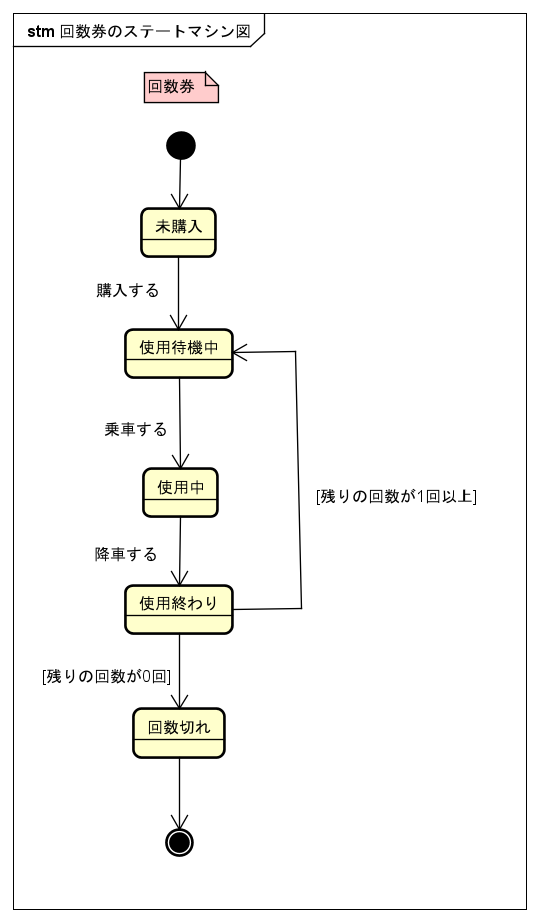
\includegraphics[width=0.9\columnwidth]{figure/8-1.png}
      \caption{回数券のステートマシン図}
      \label{fig:8-1}
  \end{minipage}
  \begin{minipage}[b]{0.49\columnwidth}
      \centering
      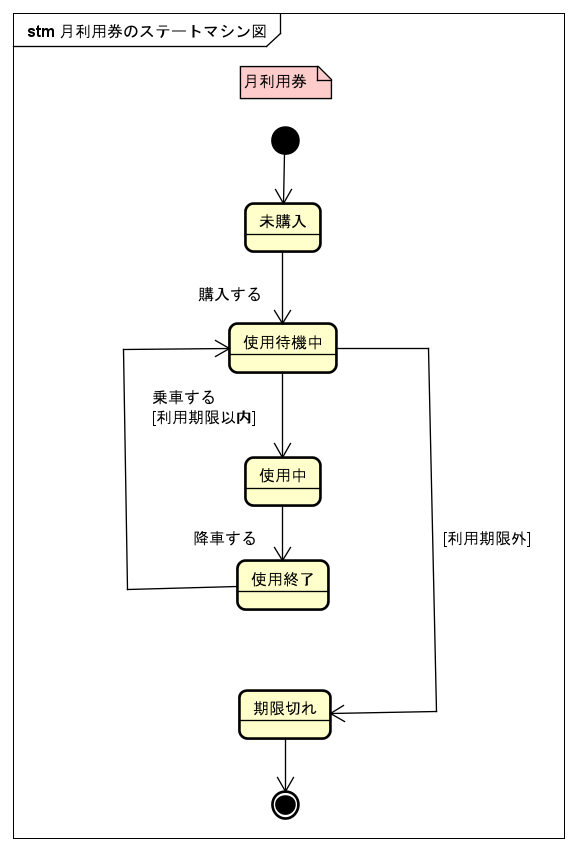
\includegraphics[width=0.9\columnwidth]{figure/8-2.png}
      \caption{利用券のステートマシン図}
      \label{fig:8-2}
  \end{minipage}
\end{figure}


\section{まとめ}
前回使用したUML図に対して複数回のレビュー訂正を行い今回のレポート作成を行った.
クラス図,シーケンス図に関してはまだ理解できていない部分があり,大きく訂正を要した.
クラス図に関しては,クラスが多すぎて図がわかりにくくなってしまった.
今後の作成でクラスの数は意識していきたい.

レビューを図を作成する事に行ったので,後の図の作成に与える影響が少なかったのは良かった.
影響が少ないというよりは,事前に作った図を元に次の図を作成したので,前の図とあっていない等のミスは減った.
今後の作成においても,図を作成するごとにレビューを行い,後の作業に影響を与えないように工夫したい.

\end{document}